% Compile with: xelatex RESEARCH_REPORT.tex
% Options for packages loaded elsewhere
\PassOptionsToPackage{unicode}{hyperref}
\PassOptionsToPackage{hyphens}{url}
\documentclass[
  11pt,
]{article}
\usepackage{xcolor}
\usepackage[margin=1in]{geometry}
\usepackage{amsmath,amssymb}
\usepackage{iftex}
\ifPDFTeX
  \usepackage[T1]{fontenc}
  \usepackage[utf8]{inputenc}
  \usepackage{textcomp} % provide euro and other symbols
\else % if luatex or xetex
  \usepackage{unicode-math} % this also loads fontspec
  \defaultfontfeatures{Scale=MatchLowercase}
  \defaultfontfeatures[\rmfamily]{Ligatures=TeX,Scale=1}
\fi
\usepackage{lmodern}
\ifPDFTeX\else
  % xetex/luatex font selection
\fi
% Use upquote if available, for straight quotes in verbatim environments
\IfFileExists{upquote.sty}{\usepackage{upquote}}{}
\IfFileExists{microtype.sty}{% use microtype if available
  \usepackage[]{microtype}
  \UseMicrotypeSet[protrusion]{basicmath} % disable protrusion for tt fonts
}{}
\makeatletter
\@ifundefined{KOMAClassName}{% if non-KOMA class
  \IfFileExists{parskip.sty}{%
    \usepackage{parskip}
  }{% else
    \setlength{\parindent}{0pt}
    \setlength{\parskip}{6pt plus 2pt minus 1pt}}
}{% if KOMA class
  \KOMAoptions{parskip=half}}
\makeatother
\usepackage{color}
\usepackage{fancyvrb}
\newcommand{\VerbBar}{|}
\newcommand{\VERB}{\Verb[commandchars=\\\{\}]}
\DefineVerbatimEnvironment{Highlighting}{Verbatim}{commandchars=\\\{\}}
% Add ',fontsize=\small' for more characters per line
\newenvironment{Shaded}{}{}
\newcommand{\AlertTok}[1]{\textcolor[rgb]{1.00,0.00,0.00}{\textbf{#1}}}
\newcommand{\AnnotationTok}[1]{\textcolor[rgb]{0.38,0.63,0.69}{\textbf{\textit{#1}}}}
\newcommand{\AttributeTok}[1]{\textcolor[rgb]{0.49,0.56,0.16}{#1}}
\newcommand{\BaseNTok}[1]{\textcolor[rgb]{0.25,0.63,0.44}{#1}}
\newcommand{\BuiltInTok}[1]{\textcolor[rgb]{0.00,0.50,0.00}{#1}}
\newcommand{\CharTok}[1]{\textcolor[rgb]{0.25,0.44,0.63}{#1}}
\newcommand{\CommentTok}[1]{\textcolor[rgb]{0.38,0.63,0.69}{\textit{#1}}}
\newcommand{\CommentVarTok}[1]{\textcolor[rgb]{0.38,0.63,0.69}{\textbf{\textit{#1}}}}
\newcommand{\ConstantTok}[1]{\textcolor[rgb]{0.53,0.00,0.00}{#1}}
\newcommand{\ControlFlowTok}[1]{\textcolor[rgb]{0.00,0.44,0.13}{\textbf{#1}}}
\newcommand{\DataTypeTok}[1]{\textcolor[rgb]{0.56,0.13,0.00}{#1}}
\newcommand{\DecValTok}[1]{\textcolor[rgb]{0.25,0.63,0.44}{#1}}
\newcommand{\DocumentationTok}[1]{\textcolor[rgb]{0.73,0.13,0.13}{\textit{#1}}}
\newcommand{\ErrorTok}[1]{\textcolor[rgb]{1.00,0.00,0.00}{\textbf{#1}}}
\newcommand{\ExtensionTok}[1]{#1}
\newcommand{\FloatTok}[1]{\textcolor[rgb]{0.25,0.63,0.44}{#1}}
\newcommand{\FunctionTok}[1]{\textcolor[rgb]{0.02,0.16,0.49}{#1}}
\newcommand{\ImportTok}[1]{\textcolor[rgb]{0.00,0.50,0.00}{\textbf{#1}}}
\newcommand{\InformationTok}[1]{\textcolor[rgb]{0.38,0.63,0.69}{\textbf{\textit{#1}}}}
\newcommand{\KeywordTok}[1]{\textcolor[rgb]{0.00,0.44,0.13}{\textbf{#1}}}
\newcommand{\NormalTok}[1]{#1}
\newcommand{\OperatorTok}[1]{\textcolor[rgb]{0.40,0.40,0.40}{#1}}
\newcommand{\OtherTok}[1]{\textcolor[rgb]{0.00,0.44,0.13}{#1}}
\newcommand{\PreprocessorTok}[1]{\textcolor[rgb]{0.74,0.48,0.00}{#1}}
\newcommand{\RegionMarkerTok}[1]{#1}
\newcommand{\SpecialCharTok}[1]{\textcolor[rgb]{0.25,0.44,0.63}{#1}}
\newcommand{\SpecialStringTok}[1]{\textcolor[rgb]{0.73,0.40,0.53}{#1}}
\newcommand{\StringTok}[1]{\textcolor[rgb]{0.25,0.44,0.63}{#1}}
\newcommand{\VariableTok}[1]{\textcolor[rgb]{0.10,0.09,0.49}{#1}}
\newcommand{\VerbatimStringTok}[1]{\textcolor[rgb]{0.25,0.44,0.63}{#1}}
\newcommand{\WarningTok}[1]{\textcolor[rgb]{0.38,0.63,0.69}{\textbf{\textit{#1}}}}
\usepackage{longtable,booktabs,array}
\usepackage{calc} % for calculating minipage widths
% Correct order of tables after \paragraph or \subparagraph
\usepackage{etoolbox}
\makeatletter
\patchcmd\longtable{\par}{\if@noskipsec\mbox{}\fi\par}{}{}
\makeatother
% Allow footnotes in longtable head/foot
\IfFileExists{footnotehyper.sty}{\usepackage{footnotehyper}}{\usepackage{footnote}}
\makesavenoteenv{longtable}
\usepackage{graphicx}
\makeatletter
\newsavebox\pandoc@box
\newcommand*\pandocbounded[1]{% scales image to fit in text height/width
  \sbox\pandoc@box{#1}%
  \Gscale@div\@tempa{\textheight}{\dimexpr\ht\pandoc@box+\dp\pandoc@box\relax}%
  \Gscale@div\@tempb{\linewidth}{\wd\pandoc@box}%
  \ifdim\@tempb\p@<\@tempa\p@\let\@tempa\@tempb\fi% select the smaller of both
  \ifdim\@tempa\p@<\p@\scalebox{\@tempa}{\usebox\pandoc@box}%
  \else\usebox{\pandoc@box}%
  \fi%
}
% Set default figure placement to htbp
\def\fps@figure{htbp}
\makeatother
\setlength{\emergencystretch}{3em} % prevent overfull lines
\providecommand{\tightlist}{%
  \setlength{\itemsep}{0pt}\setlength{\parskip}{0pt}}
\usepackage{bookmark}
\IfFileExists{xurl.sty}{\usepackage{xurl}}{} % add URL line breaks if available
\urlstyle{same}
\hypersetup{
  hidelinks,
  pdfcreator={LaTeX via pandoc}}

\title{Quant Research Lab — Research Report}
\author{}
\date{}

\begin{document}
\maketitle

\section{Quant Research Lab --- Research
Report}\label{quant-research-lab-research-report}

This report is the single narrative for the lab: alternative-data stock
screening, probability and learner diagnostics, market simulation,
technical indicators, rule-based and machine-learned trading strategies,
reinforcement learning, and agent-based market simulation.

\textbf{How to read the sections.} Where results evolved, each block is
labeled:

\begin{itemize}
\tightlist
\item
  \textbf{First implementation / first test / initial results} ---
  original design and metrics
\item
  \textbf{After improvements / updated results} --- re-runs on the
  current package, data protocol, and evaluation discipline
\end{itemize}

Where useful: \emph{X was tested and Y was received before improvements
were made.}

Figures live under \href{img/report/}{\texttt{docs/img/report/}} and
\href{img/}{\texttt{docs/img/}}. Executable detail is in
\href{../notebooks/}{\texttt{notebooks/}}. A LaTeX twin of this document
is \href{RESEARCH_REPORT.tex}{\texttt{RESEARCH\_REPORT.tex}}.

\begin{center}\rule{0.5\linewidth}{0.5pt}\end{center}

\subsection{1. Preface}\label{preface}

\textbf{Research question.} Can alternative data and machine learning
find --- and exploit --- an edge in equities, once costs and
out-of-sample evaluation are taken seriously?

The pipeline grew from a fundamentals + Glassdoor screen into a
cost-aware backtesting lab with from-scratch learners and RL. Early
trading experiments used shorter crisis-era windows and fixed
±1000-share position caps. The improved protocol standardizes on longer
train/test splits, unlevered sizing, walk-forward checks, and an
installable \texttt{quantlab} package with unit tests.

\begin{center}\rule{0.5\linewidth}{0.5pt}\end{center}

\subsection{2. Stock investment and Glassdoor alternative
data}\label{stock-investment-and-glassdoor-alternative-data}

\subsubsection{2.1 Goal}\label{goal}

Develop a database and model for stock investment decisions by compiling
public-company information (fundamentals plus employee-sourced outlook)
and turning it into auditable screens and statistical tests.

\subsubsection{2.2 Hypothesis}\label{hypothesis}

Does Glassdoor \emph{Positive Business Outlook} correlate with long-run
company ROI?

\textbf{First test.} On the 2020 research snapshots (Morningstar
fundamentals joined to Glassdoor outlook/rating), OLS and Spearman
analysis rejected the null of no association: \textbf{p ≈ 1e-10} with
\textbf{n ≈ 548}, but \textbf{r² ≈ 0.07}. Outlook behaves like a
\emph{screening factor}, not a standalone trading signal.

Caveats recorded at the time:

\begin{itemize}
\tightlist
\item
  Associational look-back returns (not a true forward prediction study)
\item
  Survivorship bias in the scraped universe
\item
  No claim of post-2020 predictive validity
\item
  Correlation is not causation
\end{itemize}

\textbf{After improvements.} The same hypothesis utilities live in
\texttt{quantlab.stats} (Cochran sample sizing, Spearman matrices with
p-values, OLS with explicit reject/fail-to-reject). Loaders in
\texttt{quantlab.data.fundamentals} clean messy CSV tokens, thousands
separators, yes/no/ESG flags, and trend labels. Notebook
\href{../notebooks/01_hypothesis_and_research_design.ipynb}{\texttt{01\_hypothesis\_and\_research\_design.ipynb}}
reproduces the verdict; provenance for the original scraper is under
\href{archive/}{\texttt{docs/archive/}}.

\subsubsection{2.3 Data pipeline}\label{data-pipeline}

\textbf{First implementation.} Web scraping assembled monthly
fundamentals + outlook tables (examples committed as
\texttt{data/2020\_09.csv}, \texttt{2020\_11.csv},
\texttt{2020\_12.csv}).

\textbf{After improvements.} A single tested loading path versions those
snapshots; prices come from Yahoo Finance with a deterministic local
cache (\texttt{quantlab.data.prices}). Notebook
\href{../notebooks/02_data_pipeline.ipynb}{\texttt{02\_data\_pipeline.ipynb}}.

\subsubsection{2.4 Screening rules}\label{screening-rules}

\textbf{First test.} Eight auditable rules compressed roughly
\textbf{1,170} names to about a \textbf{15-name} list (e.g.~AAPL, MSFT,
NVDA):

\begin{enumerate}
\def\labelenumi{\arabic{enumi}.}
\tightlist
\item
  Net income per employee ≥ \$10,000\\
\item
  Net profit margin \textgreater{} 2.57\%\\
\item
  3-, 5-, and 10-year trailing ROI all \textgreater{} 10.1\%\\
\item
  Price shows an upward trend\\
\item
  Glassdoor positive business outlook ≥ 60\%\\
\item
  Glassdoor overall rating ≥ 3.5\\
\item
  PEG ratio between 0 and 1\\
\item
  Beats S\&P 500 over 1 year and 5 years
\end{enumerate}

\textbf{After improvements.} Rules are a typed engine in
\texttt{quantlab.screening} with unit tests; notebook
\href{../notebooks/03_screening_rules.ipynb}{\texttt{03\_screening\_rules.ipynb}}.

\begin{center}\rule{0.5\linewidth}{0.5pt}\end{center}

\subsection{3. Martingale (American
roulette)}\label{martingale-american-roulette}

\subsubsection{3.1 Abstract / setup}\label{abstract-setup}

A martingale is a stochastic process where the expectation of the next
value equals the present value. Here the scenario is gambling: a
gambler's winnings form a martingale if games are fair. The practical
idea is that because you cannot lose every time, you increase the stake
after losses in anticipation of a future win that recovers prior losses.

\textbf{Setup.} Always bet on black on an American roulette wheel (0 and
00): 38 pockets, 18 black ⇒ (P(\text{win}) = 18/38 \approx 47.7\%).
Double the stake after each loss; quit at +\$80 or after 1000 sequential
bets.

Single-bet expected value (unit stake):

\[
\mathbb{E} = \tfrac{18}{38}(+1) + \tfrac{20}{38}(-1) \approx -\$0.05
\]

so the house edge is about five cents per dollar bet.

\subsubsection{3.2 Experiment 1 --- unlimited bankroll (first
test)}\label{experiment-1-unlimited-bankroll-first-test}

\textbf{Estimated probability of winning \$80 within 1000 bets.}\\
All 1000 simulations achieved +\$80 ⇒ estimated probability
\textbf{100\%}. Repeated doubling with an unlimited bank account always
recovers to the prior high and then freezes at the +\$80 target.

Figure note (first test): the first 300 bets of 10 simulations all
reached \$80 by roughly 200 sequential bets.

\textbf{Estimated expected value after 1000 bets.}\\
Because every path hits +\$80 and freezes, the mean terminal value
across simulations is \textbf{\$80}. Equivalently: the path is a
sequence of geometric progressions ending in a win that reverses losses,
then quitting at the target.

\textbf{Do mean ± SD lines reach a maximum then stabilize / converge?}\\
Yes. Once equity freezes at \$80, standard deviation → 0, so mean,
mean+SD, and mean−SD stabilize and \textbf{converge}. SD rises then
falls as more paths lock in.

Median ± SD plots behave similarly under the unlimited-bankroll freeze.

\subsubsection{3.3 Experiment 2 --- \$256 bankroll cap (first
test)}\label{experiment-2-256-bankroll-cap-first-test}

\textbf{Estimated probability of winning \$80 within 1000 bets.}\\
666 of 1000 simulations succeeded ⇒ \textbf{66.6\%}. The capital cap
blocks recovery after a deep losing streak. With single-spin win rate ≈
47.7\%, more trials would be expected to push this estimate somewhat
lower.

\textbf{Estimated expected value after 1000 bets.}\\
Paths converge near +\$80 (\textasciitilde66.6\%) or −\$256
(\textasciitilde33.3\%):

\[
0.666 \times 80 + 0.334 \times (-256) \approx -\$34.53
\]

If hit rate falls with more trials, EV becomes more negative.

\textbf{Do mean ± SD lines converge?}\\
No.~First-test plateaus were roughly: mean+SD ≈ \$126.24, mean ≈
−\$32.22, mean−SD ≈ −\$190.69, with SD ≈ \$158.46. Because a large mass
remains at −\$256, SD never approaches 0 and the bands \textbf{do not
converge}.

\subsubsection{3.4 After improvements}\label{after-improvements}

Clean API in \texttt{quantlab.sim.martingale} with seeded RNG. Re-run
(200 sims, seed 42) via \texttt{scripts/generate\_report\_assets.py}:

\begin{longtable}[]{@{}lrr@{}}
\toprule\noalign{}
Setting & Hit rate & Expected terminal \\
\midrule\noalign{}
\endhead
\bottomrule\noalign{}
\endlastfoot
Unlimited & 1.00 & 80.0 \\
Cap \$256 & 0.63 & ≈ −44.3 \\
\end{longtable}

Conclusions match the first test (sure win with infinite capital;
negative EV with a finite bankroll). Differences vs 1000-sim first-test
figures are Monte Carlo noise. See
\href{img/report/martingale_paths.png}{\texttt{martingale\_paths.png}}
and notebook
\href{../notebooks/12_martingale_and_gridworld.ipynb}{\texttt{12\_martingale\_and\_gridworld.ipynb}}.

\begin{center}\rule{0.5\linewidth}{0.5pt}\end{center}

\subsection{4. Portfolio optimization}\label{portfolio-optimization}

\subsubsection{4.1 Method}\label{method}

Maximize the Sharpe ratio of a long-only, fully invested portfolio with
SciPy SLSQP. Daily returns of the weighted book are used; the objective
is typically minimizing the negative Sharpe.

\subsubsection{4.2 First implementation}\label{first-implementation}

\textbf{Parameters}

\begin{longtable}[]{@{}ll@{}}
\toprule\noalign{}
Parameter & Value \\
\midrule\noalign{}
\endhead
\bottomrule\noalign{}
\endlastfoot
Start & 2008-06-01 \\
End & 2009-06-01 \\
Symbols & JPM, GLD, X, IBM \\
\end{longtable}

\textbf{Optimizer / portfolio results (first test)}

\begin{longtable}[]{@{}lr@{}}
\toprule\noalign{}
Metric & Value \\
\midrule\noalign{}
\endhead
\bottomrule\noalign{}
\endlastfoot
Current function value & −0.026653247 \\
Iterations & 7 \\
Function evaluations & 42 \\
Gradient evaluations & 7 \\
Allocations & ≈ {[}1, 0, 0, 0{]} (100\% JPM) \\
Sum of allocations & 1.00 \\
Sharpe ratio & −1.0939 \\
Volatility (daily) & reported alongside objective \\
Average daily return & 0.0018367 \\
Cumulative return & −0.1148 \\
\end{longtable}

Normalized optimal portfolio vs S\&P 500 was plotted for the crisis
window. The takeaway: in-sample ``optimal'' weights in a crash do not
imply a good absolute outcome --- here the Sharpe-maximizing book was
essentially all JPM and still lost money.

\subsubsection{4.3 After improvements}\label{after-improvements-1}

Notebook
\href{../notebooks/05_portfolio_optimization.ipynb}{\texttt{05\_portfolio\_optimization.ipynb}}
uses train \textbf{2016--2019} / OOS \textbf{2020--2023}, often on the
screened universe, benchmarked to SPY and equal weight
(\texttt{quantlab.portfolio}). Max-Sharpe can beat SPY out-of-sample,
but the in-sample edge decays --- the same lesson as the first test,
under a healthier evaluation protocol.

\begin{center}\rule{0.5\linewidth}{0.5pt}\end{center}

\subsection{5. Assess learners}\label{assess-learners}

\subsubsection{5.1 Abstract and
introduction}\label{abstract-and-introduction}

Compare from-scratch learners that accept tabular (non-time-series)
inputs and return continuous predictions: \textbf{decision tree},
\textbf{random tree}, \textbf{bag}, \textbf{InsaneLearner}, and
\textbf{linear regression}. Primary metric: RMSE. Later experiments also
use MAE and wall-clock time.

\textbf{Initial hypotheses (first test):}

\begin{enumerate}
\def\labelenumi{\arabic{enumi}.}
\tightlist
\item
  Increasing leaf size decreases overfitting but increases error.\\
\item
  Decision trees take longer than random trees but are more accurate,
  because they choose splits by correlation rather than at random.
\end{enumerate}

\subsubsection{5.2 Methods}\label{methods}

Data: \texttt{Istanbul.csv} (also accepted: any similar numeric matrix).
Shuffle, then \textbf{60\%} train / \textbf{40\%} test. Leaf sizes swept
\textbf{1--100} where relevant. Bagging defaults to \textbf{20} bags and
can wrap any base learner.

Split rule: decision trees pick the feature with highest absolute
correlation with the target and split at the median; random trees pick a
random feature.

\subsubsection{5.3 Experiment 1 --- leaf size vs overfitting (decision
tree)}\label{experiment-1-leaf-size-vs-overfitting-decision-tree}

Overfitting means fitting training data so closely that the model fails
on new data. Gauge it by \textbf{in-sample vs out-of-sample RMSE}.

Smaller leaf size ⇒ deeper trees ⇒ more overfit. First-test Figure 1
showed very low in-sample RMSE and high out-of-sample RMSE at small
leaves. The smallest in/out RMSE \emph{gap} occurred near \textbf{leaf
size ≈ 21}; at that point and smaller, overfit was visible. Larger
leaves constrain depth and improve generalization.

\subsubsection{5.4 Experiment 2 --- bagging}\label{experiment-2-bagging}

Bagging draws bootstrap subsets, trains a learner per bag, and averages
predictions to reduce variance. First-test Figure 2 (20 bags) showed
lower RMSE at both low and high leaf sizes than bare DT (e.g.~leaves 10,
21, 81), and a smaller in/out gap at very small leaves --- bagging
\textbf{reduces} overfit impact but does \textbf{not} eliminate it (an
overfit region remained for leaf ≲ 81). Varying bag count would not
remove that region entirely.

\subsubsection{5.5 Experiment 3 --- decision tree vs random
tree}\label{experiment-3-decision-tree-vs-random-tree}

Metrics: MAE and time to fit + query train and test (X).

Expectation: RT less accurate, often less overfit-prone in practice as a
weak learner, and faster. First-test results: DT MAE generally better;
RT up to \textbf{\textasciitilde4× faster} at small leaves, with the gap
narrowing as leaf size grows. Bagged RTs inherit the speed advantage.

\subsubsection{5.6 Non-experiment component ---
InsaneLearner}\label{non-experiment-component-insanelearner}

InsaneLearner = \textbf{20} bag learners, each a bag of \textbf{20}
linear regressors (400 linear models), implemented compactly. Linear
regression uses least squares with an intercept column.

\subsubsection{5.7 First-test summary}\label{first-test-summary}

Inverse relationship between leaf size and overfitting; RMSE gap
diagnoses overfit; bagging helps; DT vs RT is an accuracy/speed
tradeoff; \textbf{no single model wins everywhere}.

\subsubsection{5.8 After improvements}\label{after-improvements-2}

Same experiments in \texttt{quantlab.experiments} + notebook
\href{../notebooks/11_assess_learners.ipynb}{\texttt{11\_assess\_learners.ipynb}}.
Figures:
\href{img/report/learners_leaf_rmse.png}{\texttt{learners\_leaf\_rmse.png}},
\href{img/report/learners_dt_vs_rt.png}{\texttt{learners\_dt\_vs\_rt.png}}.

Synthetic \textbf{best-for-}* datasets
(\texttt{quantlab.experiments.best4}): linear targets favor OLS
(near-zero RMSE vs large tree error); axis-aligned thresholds favor
trees --- concrete proof that ``best learner'' depends on data geometry.

\begin{center}\rule{0.5\linewidth}{0.5pt}\end{center}

\subsection{6. Market simulator}\label{market-simulator}

\subsubsection{6.1 First implementation}\label{first-implementation-1}

Order-file simulator: dated BUY/SELL rows with symbol and share count;
mark portfolio value daily. Cost model: flat \textbf{commission} per
fill and fractional \textbf{impact} (buys pay more, sells receive less).

Typical early strategy settings: commission ≈ \textbf{\$9.95}, impact
\textbf{0.005}, positions in \{−1000, 0, +1000\}, start cash
\textbf{\$100,000}.

\subsubsection{6.2 After improvements}\label{after-improvements-3}

\begin{itemize}
\tightlist
\item
  \texttt{quantlab.backtest.run\_backtest} --- single-asset trade
  series\\
\item
  \texttt{quantlab.backtest.run\_orders} --- multi-symbol order logs\\
\item
  Metrics: Sharpe, max drawdown, cumulative/avg daily return, volatility
\end{itemize}

Default research costs in later notebooks: \textbf{\$1 commission +
0.1\% impact}, with \textbf{unlevered} share caps via
\texttt{affordable\_shares}.

\begin{center}\rule{0.5\linewidth}{0.5pt}\end{center}

\subsection{7. Indicators and theoretically optimal
strategy}\label{indicators-and-theoretically-optimal-strategy}

Charts historically used \textbf{adjusted close normalized to 1.0} at
the start of the window. Implementations live in
\texttt{quantlab.indicators}.

\subsubsection{7.1 Simple moving average
(SMA)}\label{simple-moving-average-sma}

SMA is the arithmetic mean of the last (n) prices:

\begin{Shaded}
\begin{Highlighting}[]
\NormalTok{prices.rolling(n).mean()}
\end{Highlighting}
\end{Shaded}

It smooths noise and lags price. Traders watch short SMA crossing above
long SMA as a possible uptrend start (and the reverse for downtrend).

\textbf{First test:} (n \in \{20, 50\}) on JPM; multiple 20/50 crosses
over \textasciitilde2 years; 20 above 50 interpreted as upward trend.

\subsubsection{7.2 Bollinger Bands}\label{bollinger-bands}

Upper/lower bands at SMA ± (width × rolling standard deviation). First
test: (n = 20), width = 2.

\begin{itemize}
\tightlist
\item
  \textbf{Squeeze} (bands close): low recent vol; often precedes a vol
  expansion, but does not by itself give direction or timing.\\
\item
  Price near lower band: often read as oversold; near upper: overbought.
  Bands alone are not sufficient trading signals (Bollinger's own
  guidance).
\end{itemize}

\textbf{\%B / band value} locates price relative to the bands.
First-test plots scaled the band value (÷10) for readability; late-2009
showed bands tightening (falling SD).

\subsubsection{7.3 Momentum}\label{momentum}

Leading rate-of-change vs price (n) periods ago (first test: (n = 20)):

\[
\text{momentum}\_t = \frac{P_t}{P_{t-n}} - 1
\]

Positive ⇒ bullish momentum. Crossing up through zero after being below
does not prove a downtrend is over --- only that it is slowing.
First-test figure: momentum spiked after the \textasciitilde2009-04
trend reversal.

\subsubsection{7.4 Exponential moving average
(EMA)}\label{exponential-moving-average-ema}

EMA weights recent prices more heavily:

\begin{enumerate}
\def\labelenumi{\arabic{enumi}.}
\tightlist
\item
  Seed with SMA\\
\item
  Multiplier (= 2/(N+1))\\
\item
  \(\mathrm{EMA}_t = P_t \cdot m + \mathrm{EMA}_{t-1}\cdot(1-m)\)\\
\end{enumerate}

\begin{Shaded}
\begin{Highlighting}[]
\NormalTok{prices.ewm(...).mean()}
\end{Highlighting}
\end{Shaded}

First test used 20- and 50-day EMA; 20 crossing above 50 as a buy cue.
EMA crosses can lag differently than SMA crosses on the same chart.

\subsubsection{7.5 Volatility}\label{volatility}

Dispersion of returns; higher vol ⇒ wider range of outcomes (riskier in
that sense). First indicator study used \textbf{7-day} rolling std of
daily returns (×2 for display); strategy work often used
\textbf{20-day}. High vol early-2009 coincided with the large downtrend.
Risk-averse traders may refuse to trade when vol is extreme; others
combine high vol with trend direction as a signal.

\subsubsection{7.6 Signal research (after
improvements)}\label{signal-research-after-improvements}

Notebook
\href{../notebooks/04_signal_research.ipynb}{\texttt{04\_signal\_research.ipynb}}:
information coefficients vs forward returns are consistent for some
mean-reversion features but tiny (\textbf{\textbar IC\textbar{}
\textless{} 0.1}), so \textbf{costs dominate}.

\subsubsection{7.7 Theoretically optimal strategy
(TOS)}\label{theoretically-optimal-strategy-tos}

\textbf{Assumptions.} Perfect foresight of tomorrow's close; no bankroll
limit; trades at adjusted close; at most one trade/day; positions in
\{−1000, 0, +1000\}; \textbf{zero} commission and impact.

\textbf{Construction (first test).} Mark each day +1/−1 by whether the
next close is higher/lower. When that sign flips, trade to flip between
long and short (share deltas up to ±2000 while net holdings stay in
\{−1000, 0, +1000\}).

\textbf{Window:} JPM, 2008-01-01 → 2009-12-31, \$100,000 start.

\textbf{Benchmark:} buy 1000 shares day one and hold (normalized to
1.0).

\textbf{First-test performance}

\begin{longtable}[]{@{}lrr@{}}
\toprule\noalign{}
Metric & TOS & Benchmark \\
\midrule\noalign{}
\endhead
\bottomrule\noalign{}
\endlastfoot
Sharpe ratio & 13.3228 & 0.1569 \\
Cumulative return & 5.7861 & 0.0123 \\
Stdev of daily returns & 0.0045 & 0.0170 \\
Average daily return & 0.0038 & 0.0002 \\
Final value & \$678,610 & \$101,230 \\
\end{longtable}

Benchmark stayed relatively flat; TOS trended strongly upward --- an
upper bound, not a tradable policy.

\textbf{After improvements.} \texttt{theoretically\_optimal\_trades} in
\texttt{quantlab.strategies}; notebook 06 uses it as a ceiling.
Illustration:
\href{img/report/tos_ceiling.png}{\texttt{tos\_ceiling.png}}.

\begin{center}\rule{0.5\linewidth}{0.5pt}\end{center}

\subsection{8. Q-learning}\label{q-learning}

\subsubsection{8.1 First test --- grid
worlds}\label{first-test-grid-worlds}

Tabular Q-learning (optional \textbf{Dyna} replay) on discrete mazes
(\texttt{data/gridworlds/}). Actions: N/E/S/W. Rewards: step penalty,
large penalty for pits, positive reward at goal. The agent learns a path
from start to goal.

\subsubsection{8.2 After improvements --- trading
application}\label{after-improvements-trading-application}

Same \texttt{QLearner} drives \texttt{TradingEnvironment}:
quantile-binned indicators + position in the state; reward = position ×
next return − impact. Notebook
\href{../notebooks/08_rl_trading_agent.ipynb}{\texttt{08\_rl\_trading\_agent.ipynb}}:
learns a conservative policy but is too coarse to beat buy-and-hold on
MSFT OOS. Notebook
\href{../notebooks/12_martingale_and_gridworld.ipynb}{\texttt{12\_martingale\_and\_gridworld.ipynb}}
keeps maze training available.

\begin{center}\rule{0.5\linewidth}{0.5pt}\end{center}

\subsection{9. Strategy evaluation}\label{strategy-evaluation}

\textbf{Initial hypothesis (first test):} Manual Strategy beats
Benchmark \textbf{in-sample}; Strategy Learner beats Manual.

\subsubsection{9.1 Indicators used for
strategies}\label{indicators-used-for-strategies}

Same family as §7 (SMA 20/50, Bollinger (n=20), width 2, momentum 20,
volatility 20-day ×2 for display/signals). Prices forward- then
back-filled and normalized to 1.0 at start for the first-test charts.

\subsubsection{9.2 Manual strategy --- creation and signals (first
implementation)}\label{manual-strategy-creation-and-signals-first-implementation}

\textbf{Windows:} in-sample 2008-01-01 → 2009-12-31; out-of-sample
2010-01-01 → 2011-12-31. Symbol JPM. Holdings constrained to \{−1000, 0,
+1000\}.

Actions sum component votes: sum \textgreater{} 0 ⇒ buy, sum \textless{}
0 ⇒ sell, 0 ⇒ flat. Multiple indicators hedge single-indicator failure
and allow trading vs pure hold.

\textbf{+1 / buy} when any of:

\begin{enumerate}
\def\labelenumi{\arabic{enumi}.}
\tightlist
\item
  20-day SMA crosses \textbf{above} 50-day SMA (today above, yesterday
  below).\\
\item
  Price crosses \textbf{above} the lower Bollinger band (today above,
  yesterday below).\\
\item
  Momentum crosses \textbf{above} zero (today \textgreater{} 0,
  yesterday \textless{} 0, with the prior-day stability check used in
  the first implementation).
\end{enumerate}

\textbf{−1 / sell} when any of:

\begin{enumerate}
\def\labelenumi{\arabic{enumi}.}
\tightlist
\item
  20-day SMA crosses \textbf{below} 50-day SMA.\\
\item
  Price crosses \textbf{below} the upper Bollinger band.\\
\item
  Momentum crosses \textbf{below} zero (symmetric to the buy rule).
\end{enumerate}

Example: votes (+1, −1, 0) sum to 0 ⇒ no trade.

\subsubsection{9.3 Manual vs benchmark --- first-test
performance}\label{manual-vs-benchmark-first-test-performance}

In-sample: Manual beat Benchmark (as designed). Out-of-sample: Manual
\textbf{worse} than Benchmark --- thresholds tuned on in-sample did not
transfer. ``Past performance doesn't guarantee future performance.''

\begin{longtable}[]{@{}lrrrr@{}}
\toprule\noalign{}
Metric & Manual (In) & Bench (In) & Manual (Out) & Bench (Out) \\
\midrule\noalign{}
\endhead
\bottomrule\noalign{}
\endlastfoot
Sharpe & 0.188 & 0.153 & −1.4569 & −0.2636 \\
Cumulative return & 0.034 & 0.01 & −0.3847 & −0.0853 \\
Stdev daily return & 0.0151 & 0.017 & 0.00997 & 0.0085 \\
Avg daily return & 0.000179 & 0.00016 & −0.0009 & −0.00014 \\
Number of trades & 41 & 2 & 40 & 2 \\
Final value & \$103,340.80 & \$100,819.25 & \$61,517.55 & \$91,273.10 \\
\end{longtable}

Extra trades explain in-sample outperformance vs a static hold; the same
activity hurt out-of-sample.

\subsubsection{9.4 Strategy learner (first
implementation)}\label{strategy-learner-first-implementation}

\textbf{Features:} same indicators as Manual (incl.~20/50 SMA ratio,
Bollinger \%B, momentum, volatility). \textbf{Target:} 5-day percent
return, discretized to \{−1, 0, +1\} with thresholds that include
impact. Missing features filled with 0.

\textbf{Model:} BagLearner of Random Trees --- \textbf{20 bags},
\textbf{leaf size 6} (larger leaf to limit degradation). Train
2008--2009; test 2010--2011.

\subsubsection{9.5 Experiment 1 --- Manual vs Learner vs Benchmark
(first
test)}\label{experiment-1-manual-vs-learner-vs-benchmark-first-test}

Commission \textbf{9.5}, impact \textbf{0.005}, \$100k start, ±1000
shares, fixed RNG seed.

Hypothesis: Learner beats Manual --- \textbf{supported} in- and
out-of-sample vs Manual. Out-of-sample, \textbf{Benchmark still beat the
Learner}; all three finished below start in that OOS window. Without a
seed, RT bags would not reproduce exactly; other OOS windows might
change rankings.

\textbf{In-sample table (first test)}

\begin{longtable}[]{@{}lrrr@{}}
\toprule\noalign{}
Metric & Strategy Learner & Manual & Benchmark \\
\midrule\noalign{}
\endhead
\bottomrule\noalign{}
\endlastfoot
Sharpe & 3.6 & 0.188 & 0.153 \\
Cumulative return & 1.816 & 0.034 & 0.01 \\
Stdev daily return & 0.009 & 0.0151 & 0.017 \\
Avg daily return & 0.0021 & 0.000179 & 0.00016 \\
Number of trades & 117 & 41 & 2 \\
Final value & \$281,056.30 & \$103,340.80 & \$100,819.25 \\
\end{longtable}

In-sample, the Learner had the best return and Sharpe with the
\textbf{lowest} daily vol while trading the \textbf{most} --- classic
in-sample success that did not fully carry OOS against buy-and-hold.

\subsubsection{9.6 Experiment 2 --- impact sensitivity (first
test)}\label{experiment-2-impact-sensitivity-first-test}

Commission \textbf{0}; impacts \textbf{0, 0.002, 0.004, 0.006}.
Hypothesis: larger impact ⇒ lower final value (impact is a cost).
Generally true for cum return / avg daily return / final value; not
perfectly monotone at tiny impact steps because of random trees. Higher
impact tended to reduce Sharpe. At impact ≃ 0.02, trades became minimal;
high enough impact can yield \textbf{no} trades.

\textbf{In-sample impact table (first test)}

\begin{longtable}[]{@{}lrrrr@{}}
\toprule\noalign{}
Impact & 0 & 0.002 & 0.004 & 0.006 \\
\midrule\noalign{}
\endhead
\bottomrule\noalign{}
\endlastfoot
Sharpe & 3.676 & 3.857 & 3.901 & 3.535 \\
Cumulative return & 1.92 & 2.023 & 2.043 & 1.776 \\
Stdev daily & 0.00938 & 0.00921 & 0.00916 & 0.0093 \\
Avg daily return & 0.00217 & 0.00223 & 0.00225 & 0.00207 \\
Number of trades & 93 & 109 & 103 & 112 \\
Final value & \$292,030 & \$302,036 & \$303,881 & \$276,948 \\
\end{longtable}

\subsubsection{9.7 After improvements}\label{after-improvements-4}

Protocol: \textbf{MSFT}, train \textbf{2016--2019}, OOS
\textbf{2020--2023}, \$100k, unlevered shares, \textbf{\$1 + 0.1\%}
impact. Manual rules use vote thresholds in \texttt{ManualRuleStrategy};
ML uses bagged random trees in \texttt{MLTradingStrategy}. Walk-forward
yearly checks show the ML edge is \textbf{not} year-consistent.

\begin{longtable}[]{@{}
  >{\raggedright\arraybackslash}p{(\linewidth - 8\tabcolsep) * \real{0.1562}}
  >{\raggedleft\arraybackslash}p{(\linewidth - 8\tabcolsep) * \real{0.2969}}
  >{\raggedleft\arraybackslash}p{(\linewidth - 8\tabcolsep) * \real{0.1250}}
  >{\raggedleft\arraybackslash}p{(\linewidth - 8\tabcolsep) * \real{0.2188}}
  >{\raggedleft\arraybackslash}p{(\linewidth - 8\tabcolsep) * \real{0.2031}}@{}}
\toprule\noalign{}
\begin{minipage}[b]{\linewidth}\raggedright
Strategy
\end{minipage} & \begin{minipage}[b]{\linewidth}\raggedleft
Cumulative return
\end{minipage} & \begin{minipage}[b]{\linewidth}\raggedleft
Sharpe
\end{minipage} & \begin{minipage}[b]{\linewidth}\raggedleft
Max drawdown
\end{minipage} & \begin{minipage}[b]{\linewidth}\raggedleft
Final value
\end{minipage} \\
\midrule\noalign{}
\endhead
\bottomrule\noalign{}
\endlastfoot
ML learner (bagged random trees) & \textbf{+185.4\%} & \textbf{1.02} &
\textbf{−27.0\%} & \textbf{\$285,412} \\
Buy \& hold & +143.0\% & 0.85 & −37.2\% & \$242,714 \\
Manual rules & +33.1\% & 0.38 & −45.4\% & \$133,046 \\
Q-learner & +6.1\% & 0.17 & −31.4\% & \$106,103 \\
\end{longtable}

Impact grids remain in notebook 06. Limitations: single-symbol strategy
evaluation, simple cost model, 2020 fundamentals vintage.

\begin{figure}
\centering
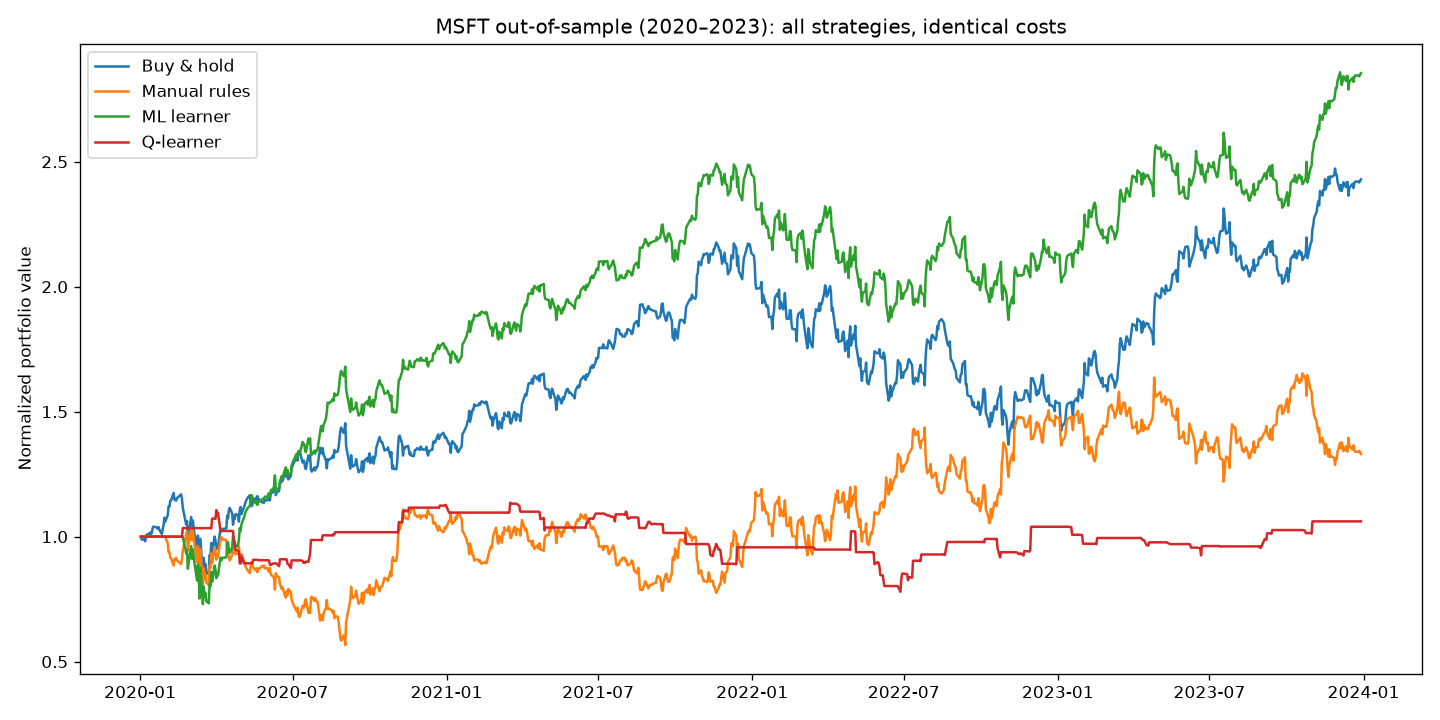
\includegraphics[keepaspectratio,alt={Final scorecard}]{img/09_final_scorecard.png}
\caption{Final scorecard}
\end{figure}

\begin{center}\rule{0.5\linewidth}{0.5pt}\end{center}

\subsection{10. ABIDES market
simulation}\label{abides-market-simulation}

\subsubsection{10.1 First implementation --- agent
design}\label{first-implementation-agent-design}

Custom agent in the Agent-Based Interactive Discrete Event Simulation
environment (EMA mid-price momentum + inventory-aware quoting):

\begin{enumerate}
\def\labelenumi{\arabic{enumi}.}
\tightlist
\item
  On wake: cancel resting orders; fetch spread / book.\\
\item
  Compare fast vs slow mid-price EMAs → buy / sell / flat momentum
  status.\\
\item
  Size and price using depth-weighted mid estimates and recent bid--ask
  spread volatility; inventory skew raises bids when flat/cash-heavy and
  lowers asks when long.\\
\item
  Place an order only when momentum and inventory logic agree; pause
  after fills to avoid over-leverage / order spam.\\
\item
  Flatten within \textasciitilde5 minutes of the close.
\end{enumerate}

\subsubsection{10.2 After improvements}\label{after-improvements-5}

Kernel vendored under
\href{../third_party/abides/}{\texttt{third\_party/abides/}} (see
\texttt{PROVENANCE.md} and upstream LICENSE). Strategy logic also as
testable pure functions in \texttt{quantlab.abides\_agent}. Notebook
\href{../notebooks/10_abides_market_simulation.ipynb}{\texttt{10\_abides\_market\_simulation.ipynb}}
and \texttt{quantlab.abides\_runner}
(\texttt{pip install -e ".[abides]"}).

\begin{center}\rule{0.5\linewidth}{0.5pt}\end{center}

\subsection{11. Unified conclusions}\label{unified-conclusions}

\begin{enumerate}
\def\labelenumi{\arabic{enumi}.}
\tightlist
\item
  \textbf{Glassdoor outlook} associates with historical ROI weakly
  (screening factor, not standalone alpha).\\
\item
  \textbf{Finite-bankroll martingales} have negative expected value
  despite frequent small wins.\\
\item
  \textbf{Learner choice} depends on leaf size, bagging, and data
  geometry.\\
\item
  \textbf{TOS} shows how large a frictionless edge looks; real
  strategies must clear costs.\\
\item
  \textbf{Hand rules} overfit short in-sample windows; \textbf{bagged
  trees} can beat buy-and-hold on a modern OOS window but fail
  walk-forward consistency.\\
\item
  \textbf{Tabular RL} learns sensible low-risk behavior, not a
  benchmark-beating policy under the current state design.\\
\item
  \textbf{ABIDES} remains the path for microstructure-style agent
  experiments.
\end{enumerate}

\textbf{Next steps} (notebook 09): cross-sectional ML on the full
screen, deeper RL, fresher alternative data, richer execution realism.

\begin{center}\rule{0.5\linewidth}{0.5pt}\end{center}

\subsection{References}\label{references}

\begin{enumerate}
\def\labelenumi{\arabic{enumi}.}
\tightlist
\item
  Hayes, A. (2020, August 28). Bollinger Band®.
  https://www.investopedia.com/terms/b/bollingerbands.asp\\
\item
  Hayes, A. (2020, September 10). Exponential Moving Average (EMA).
  https://www.investopedia.com/terms/e/ema.asp\\
\item
  Hayes, A. (2020, September 22). Simple Moving Average (SMA)
  Definition. https://www.investopedia.com/terms/s/sma.asp\\
\item
  Staff, I. (2020, August 28). Momentum Indicates Stock Price Strength.
  https://www.investopedia.com/articles/technical/081501.asp\\
\item
  Woods, G. (2019, September 26). Trading with the Bollinger Band
  Squeeze. https://www.tradingsetupsreview.com/bollinger-squeeze/\\
\item
  Byrd, D., Hybinette, M., \& Balch, T. \emph{ABIDES: Towards
  High-Fidelity Market Simulation for AI Research}. arXiv:1904.12066.
\end{enumerate}

\end{document}
